\chapter{Projekt i jego implementacja}

Założeniami projektu opisanego w ninejszej pracy było stworzenie prototypu
oprogramowania umożliwiającego wykrywanie ataków DDoS w sieciach SDN oraz, co
ważniejsze, dającego się łatwo skalować w celu zwiększenia jego wydajności.
Wykorzystanie właściwej archtiektury rozwiązania oraz dobór odpowiednich
technologii do jego implementacji umożliwiły osiągnięcie zamierzonych celów.

\section{Architektura rozwiązania wykrywania ataku DDoS}

Projektując tytułowe rozwiązanie należało wziąć pod uwagę następujące czynniki:
\begin{itemize}
  \item umiejscowienie komponentu z oprogramowaniem w architekturze sieci SDN
  \item uzyskanie odpowiednich danych z sieci, pozwalających na wykrycie ataku
  \item wydajność działania oprogramowania
\end{itemize}

Oprogramowanie zostało zaprojektowane do działania na południowym interfejsie
architektury sieci SDN. Takie umiejscowienie dostarcza wielu możliwości.
Pierwszą z nich jest to, że oprogramowanie może być częścią przełącznika,
kontrolera lub działać na osobnym węźle. Dodatkowo oprogramowanie ma dostęp do
danych wymienianych pomiędzy przełącznikiem, a kontrolerem. Możliwość analizy
tychże danych była podstawą do implementacji algorytmu do wykrywania ataków DDoS
w sieci. Szczegóły dotyczące algorytmu zostały opisane w późniejszym rozdziale
ninejszej pracy. 

Oprogramowanie zaimplementowano z myślą o działaniu na osobnym węźle,
ponieważ dzięki takiemu podejściu, w przypadku równoległego działania
oprogramowania, liczba jego instancji jest niezależna od liczby przełączników
lub kontrolerów. Pozwala to na bardziej elastyczne skalowanie horyzontalne
oprogramowania w celu zwiększenia jego wydajności. Ponadto zarówno przełączniki
jak i kontroler nie są świadome obecności dodatkowego komponentu pomiędzy nimi,
co pozwala uniknąć dodatkowego narzutu związanego z konfiguracją sieci SDN.

Podstawowa topologia sieci SDN wraz z umiejscowionym komponentem reprezentującym
zaimplementowane oprogramowanie (\textit{sample component}) została
przedstawiona na Rys. \ref{fig:sdn_epc_flow}. 

\begin{figure}[h]
\centering
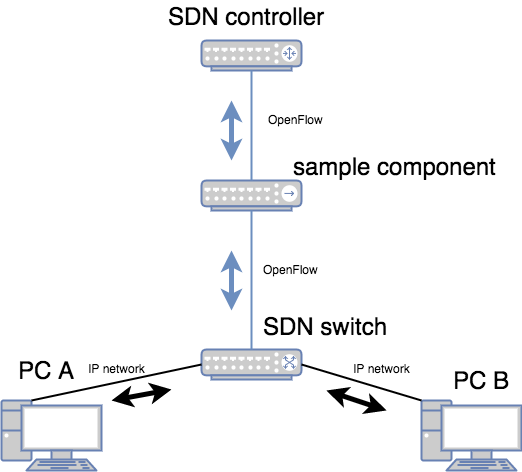
\includegraphics[width=\textwidth]{sdn_epc_flow}
\caption{Schemat podstawowej topologii sieciowej z umiejscowionym komponentem
  implementującym rozwiązanie projektowe}
\label{fig:sdn_epc_flow}
\end{figure}

Jak przedstawiono na Rys. \ref{fig:sdn_epc_flow} węzły końcowe
(\textit{PC N}) komunikują się ze sobą z wykorzystaniem przełącznika sieci SDN
(\textit{SDN switch}), a cały ruch pomiędzy przełącznikiem, a kontrolerem
(\textit{SDN controller}) przepływa przez wspomniany komponent implementujący
rozwiązanie projektowe (\textit{sample component}). 

Topologia zaprezentowana na Rys \ref{fig:sdn_epc_flow}, jak wspomniano, jest
tolopogią najbardziej podstawową, odpowiednią do wykorzystania przybliżonego
rozwiązania. Możliwe jest również zastosowanie go w bardziej
rozbudowanej sieci, składającej się z większej liczby węzłów końcowych, 
przełączników oraz kontrolerów. W takim przypadku, można użyć kilku instancji
równlegle działającego oprogramowania (komponentu), w celu zwiększenia
wydajności systemu, rozumianego jako kilka współpracujących ze sobą instancji.
System taki, można zastosować do większych, pracujących pod większym obciążeniem
sieci.

\section{Wybór odpowiednich technologii do implementacji systemu}

Podstawowym kryterium wyboru odpowiednich technologii do realizacji projektu
była wydajność. Wydajność jest rozumiana jako ilość pracy wykonana przez system
komputerowy w danym czasie i przy wykorzystaniu danej ilości zasobów
obliczeniowych \cite{distrforfunandprof}. Na potrzeby projektu, odpowiedni
poziom wydajności został zapewniony dzięki doborze techologi, które wspierają
koncepcję programowania współbieżnego, czyli możliwość wykonywania się
oprogramowania z wykorzytaniem wielu wątków fizycznych procesora maszyny, na
której zostało ono uruchomione. Ponadto przy wyborze technologi, kierowano się
również natywnym wsparciem dla możliwosći dystrybucji oprogramowania na wiele
maszyn fizycznych, czyli, innymi słowy, wsparciem dla budowania systemów
rozproszonych. Możliwość rozbudowy systemu z wykorzystaniem wielu maszyn jest
kluczowa, ponieważ nawet dysponując technolgią ze wsparciem dla programowania
współbieżnego, istnieje granica dla rozbudowy zasobów sprzętowych, dlatego w
pewnym momencie koniecznym jest budowa systemu rozproszonego
\cite{distrforfunandprof}. 

Wykorzystanie technolgii, która umożliwa programowanie współbieżne oraz wspiera
budowę systemów rozproszonych, umożliwiło taką implementację projeku, która
pozwala na łatwe oraz efektywne jego skalowanie, celem zwiększenia wydajności.

Technologiami, które spełniają wszystkie wyżej wymienione wytyczne są funkcyjne
języki programowania Erlang oraz Elixir. Oba te języki działają na Maszynie
Wirtualnej Erlanga (\textit{BEAM}). Elixir jest nowoczesną wersją
Erlanga, dopasowaną do dzisiejszych standardów. Oferuje on szereg nowoczesnych,
ułatwiających pracę programistyczną narzędzi, których Erlang nie posiada. W
rzeczywistości Elixir jest Erlangową aplikacją działającą na Maszynie Wirtualnej
Erlanga \cite{thebeambook}.

Maszyna Wirtualna Erlanga wprowadza model aktorów
\footnote{https://en.wikipedia.org/wiki/Actor\_model}, dzięki czemu posiada
natywne wsparcie dla programowania równoległego. Ponadto \textit{BEAM} zapewnia
również wsparcie dla budowy systemów rozproszonych \cite{lyserlang}. Dzięki
temu, języki Erlang oraz Elixir są odpowiednie do budowy wydajnych,
niezawodnych, systemów rozproszonych. Z tych właśnie powodów, wspomniane
technologie zostały wykorzystane do budowy projektu przedstawionego w niniejszej
pracy.

\section{Algorytm detekcji ataku DDoS} \label{algorithm}

Alogrytm detekcji ataku, zaimplementowany na potrzeby opisywanego projektu
bazuje na entropii pakietów przepływających przez sieć SDN. Entropia pakietów
rozumiana jest jako ich losowość. Im większa entropia tym większa losowość
pakietów i odwrotnie \cite{mainddosarticle}. Entropia jest wyliczana na
podstawie wzoru \ref{equ:entropy} \cite{mainddosarticle}.

\begin{equation}
H = -\sum_{i=1}^{n}p_{i}\log_{}p_{i}
\label{equ:entropy}
\end{equation}
gdzie $H$ oznacza wartość entropii, $n$ liczbę pakietów (tzw. rozmiar okna),
a $p_{i}$ wartość prawdopodbieństwa wystąpienia poszczególnego pakietu.

Wspomniany rozmiar okna jest defininowany jako ilość pakietów, dla których
jest obliczana entropia. Rozważając przypadek dla okna o rozmiarze 50, przy
założeniu, że każdy element okna wystąpił dokładnie jeden raz, wartośc entropi
obliczonej zgodnie ze wzorem \ref{equ:entropy} wyniesie 1,70. Natomiast w
przypadku, gdy jeden z elementów okna pojawi się dokładnie dziesięć razy, a
pozostałe 40 elementów tylko raz, entropia wyniesie 1,47.

Przedstawiona zależność entropii i losowości pakietów została wykorzystana do
wykrywania ataku DDoS. Atak DDoS zazwyczaj skupia się na jednym, wybranym węźle
końcowym, czyli w przypadku ataku większość pakietów w sieci zawiera jeden,
konkretny adres docelowy. W takiej sytuacji losowość pakietów w sieci spada, a
co za tym idzie, spada również entropia. Bazując na tym fakcie, można ustalić
limit wartości entropii poniżej którego, uznaje się, że w sieci nastąpił atak
DDoS. 

Zaimplementowany algorytm analizuje adresy docelowe pakietów \textit{IP}
przepływających przez sieć, tj. zlicza ilość wystąpień każdego adresu docelowego
zawartego w badanych pakietach \textit{IP}. Gdy ilość przeanalizwanych pakietów
jest równa rozmiarowi okna obliczana jest entropia. W tym celu wykorzystywane są
równania: \ref{equ:entropy}, \ref{equ:window} \cite{mainddosarticle} oraz
\ref{equ:packet_prob} \cite{mainddosarticle}.

\begin{equation}
W = \{(x_{1},y_{1}),(x_{2},y_{2}),(x_{3},y_{3}),...\}
\label{equ:window}
\end{equation}

\begin{equation}
p_{i} = \frac{y_{i}}{n}
\label{equ:packet_prob}
\end{equation}

Równanie \ref{equ:window} przedstawia reprezentację okna ($W$), gdzie $x_{i}$
oznacza dany docelowy adres \textit{IP}, a $y_{i}$ liczbę jego wystąpień w danym
oknie. Równanie \ref{equ:packet_prob} pozwala wyliczyć prawdopodobieństwo
danego pakietu ($p_{i}$), gdzie $y_{i}$ oznacza liczbę wystąpień danego adresu
\textit{IP}, a $n$ liczbę wszystkich pakietów w oknie ($W$).
Jeśli obliczona wartość entropii dla określonej liczby okien z rzędu
(rekomendowana liczba okien  wynosi 5 \cite{mainddosarticle}) jest mniejsza niż
zadana wartość, uznaje się, że w sieci nastąpił atak. 

\section{Aplikacja wykrywania ataku DDoS}

Aplikacja \textit{sdn\_epc} \footnote{https://github.com/mkacper/sdn\_epc}
(\textit{Software Defined Networking Elixir Pseudo Controller}) została w
głównej mierze wykonana przy użyciu języka programowania Elixir, aczkolwiek
wykorzystuje również kod napisany w Erlangu (głównie do interakcji z
zewnętrznymi Erlangowymi bibliotekami). Użycie dwóch języków jednocześnie było
możliwe ponieważ, jak wspomniano we wcześniejszym rozdziale, oba te języki
finalnie są kompilowne do tego samego kodu binarnego i wykonują się na tej samej
maszynie wirtualnej (\textit{BEAM}). Ponadto kompilator Elixira potrafi również 
kompilować kod Erlanga.

\subsection{Zasada działania aplikacji}

Jak przedstawiono na Rys. \ref{fig:sdn_epc_flow} strona
\pageref{fig:sdn_epc_flow} aplikacja \textit{sdn\_epc} została zaprogramowana
jako osobny komponent, działający na osobnej maszynie, połączony bezpośrednio z
przełącznikami oraz z kontrolerm sieci SDN. Komponenty te komunikują się ze
sobą z wykorzystaniem protokołu \textit{OpenFlow}. W przedstawionej konfiguracji,
cały ruch sieciowy pomiędzy przełącznikami, a kontrolerem przepływa przez
komponent \textit{sdn\_epc}. Umożliwienie połączenia systemu Elixirowego z
komponentami sieciowym, z wykorzystaniem \textit{OpenFlow} wymaga umiejętności
obsługi tego protokołu przez aplikację \textit{sdn\_epc}. W tym celu
wykorzystane zostały Erlangowe biblioteki \textit{of\_protocol}
\footnote{https://github.com/FlowForwarding/of\_protocol} oraz
\textit{ofs\_handler} \footnote{https://github.com/FlowForwarding/ofs\_handler}.

Przepływający przez komponent \textit{sdn\_epc} ruch \textit{OpenFlow} jest
analizowany na potrzeby algorytmu opisanego w rozdziale \ref{algorithm}.
Analizowane są wiadomości \textit{PACKET\_IN} protokołu \textit{OpenFlow}, a
konkretnie docelowe adresy pakietów \textit{IP} przesyłanych jako część
wiadomości \textit{PACKET\_IN}. Wyniki zapisywane są w rozproszonej bazie danych
(\textit{Mnesia}) \footnote{hhttp://erlang.org/doc/apps/mnesia/index.htm}
dostarczanej razem ze standardową dystrybucją Erlanga. Następnie zapisane
wyniki wykorzystywane są do działania wspomnianego algorytmu.

\subsection{Wydajność aplikacji}

Architektura aplikacji \textit{sdn\_epc} uwzględnia możliwosci jakie daje
Maszyna Wirtualna Erlanga w zakresie programowania równoległego oraz dystrybucji
oprogramowania na wiele węzłów. Dzięki wsparciu dla programowania równoległego
aplikacja \textit{sdn\_epc} może w tym samym czasie obsługiwać wiele (w
rzeczywistości tyle ile wątków może obsłużyc maszyna, na której działa
aplikacja) podłączonych do niej przełączników sieci SDN. \textit{BEAM} wprowadza
koncepcję procesów, w kontekście których, wykonuje się każdy kawałek
Erlangowego/Elixirowego kodu. Koncepcja ta jest podobna do koncepcji procesów
systemowych - wykonują się one na wszystkich procesorach (jeden proces na
jednym procesorze w tym samym czasie), ale mają znacznie mniejszy narzut w
kontekście zużycia zasobów systemowych niż tradycyjne procesy \cite{progelixir}.
Wykorzystując koncepcję procesów, kod odpowiedzialny za obsługę przełączników
podłączonych do aplikacji wykonuje się w osobnym procesie dla każdego z nich.
Innym słowy, każdy przełącznik jest obsługiwany przez osobny, dedykowany dla
niego proces, co umożliwa jednoczesną obsługę wielu przełączników.

Aplikacja \textit{sdn\_epc} może działać w klastrze, dzięki czemu możliwe jest
zwiększenie jej wydajności. Do działania w klastrze aplikacja wykorzystuje
wbudowany w \textit{BEAM}'a mechanizm zwany \textit{Erlang Distributed}
\footnote{http://erlang.org/doc/reference\_manual/distributed.html}. Mechnizm
ten umożliwa komunikowanie się ze sobą wielu węzłów (Maszyn Wirtualnych
Erlanga) \cite{erldocs}. Dzięki wspomnianej koncepcji procesów rozproszenie
oprogramowania na wiele węzłów nie stanowi problemu, ponieważ z punktu widzenia
Erlangowego systemu nie ma znaczenia na którym węźle wykonuje się dany proces
(procesy komunikują się w ten sam sposób niezależnie od węzła na którym
działają \cite{erldocs}). Jednakże w przypadku działania w aplikacji
\textit{sdn\_epc} w klastrze, pojawił się problem z synchronizacją stanu (danych
zapisywanych na potrzeby algorytmu do wykrywania ataku DDoS) pomiędzy węzłami.

Silna konsystencja (z ang. \textit{strong consistency}) w nomenklaturze systemów
rozprosznych oznacza, że wszystkie węzły widzą dokładnie ten same dane w
tym samym czasie \cite{distrforfunandprof}. Algorytm zaimplementowany w
aplikacji \textit{sdn\_epc} wymaga takiego własnie poziomu konsystencji danych,
ponieważ tylko jeden węzeł w tym samy czasie powinien wykryć atak i ewentulanie
podjąć jakąś akcję. Baza danych \textit{Mnesia}, zastosowana na potrzeby
algorytmu umożliwia takie jej wykorzystanie, które pozwala na osiągniecie silnej
konsystencji danych. W tym celu wykorzystano koncepcję transakcji, które
wprowadza \textit{Mnesia}. Transakcję odgrywają rolę globalnych \textit{mutex}'ów
(z ang. \textit{mutual exclusion}
\footnote{https://en.wikipedia.org/wiki/Mutual\_exclusion}), zapobiegając
równoczesnemu dostępowi różnych węzłów \textit{sdn\_epc} do danych. Zastosowanie
transakcji umożliwiło poprawną implementację algortymu dla przypadku, gdy
aplikacja \textit{sdn\_epc} działa w klastrze.